\section{Framework}
\label{sec:algo}

%\KZ{Put comments in all algos to say what the input parameters are.}

In this section, we introduce a novel image clustering framework
based on conceptualization of contexts.
Our input is a image search query and
a set of images returned by this query along with their hosting HTML pages.
Our output is a number of clusters of images, each containing images
of the same entity and each tagged with a concise list of
most representative concepts. For example, the first
cluster of \figref{fig:demo-bean} is tagged with ``Mr. Bean'', 
``Rowan Atkinson'', etc.

%First, we extract related context
%using a refined sibling based algorithm. Second, with those high quality
%context, we perform conceptualization process on the context
%to represent plain texts with a set of concepts.
%Third, we cluster images using a tri-stage clustering algorithm.

\begin{figure}[th]
\begin{center}
\centering
\includegraphics[width=\columnwidth]{framework_novisual.eps}
\caption{The Architecture of Image Clustering by Conceptualization}
\label{fig:frame}
\end{center}
\vspace*{-5mm}
\end{figure}

The architecture of our framework is shown in \figref{fig:frame}.
The framework is divided into two parts: online and offline components.
The offline components extract the meta data of the image and
conceptualize all of the text in the source page. Online components 1) extract
the surrounding text context of the image and query from the conceptualized source page and
then uses concepts in the context to construct the concept vector
representation of the image context; and 2) cluster the images using
a tri-stage clustering algorithm. We put the context extraction process
online because the query context cannot be extracted before the user
submit the query. In the following sub-sections, we introduce the technical
details of each component in our framework.

\subsection{Context Extraction}
%\cite{VIPS}
%The context of an image is any textual information about the image
%in the original web page. The context often surrounds the image on the
%rendered page and contains information related to the image.
%Besides the image, we also use the query string as a signal to search
%for additional context. 
The context extraction process can be described as a function
that takes as input a web page, a image which is embedded in the page
and a query string which produces the page and the image, 
and returns the context which includes two parts:
the image tag context and the plain text context.
Image tag context is essentially the URL and the
ALT name (label) of the image in the <IMG> tag. 
The plain text context comes from two sources, 
one from the text surrounding the image
and the other from the text surrounding the query string.

% The two parts, image context and query string context extraction
% are introduced respectively.

% This can be formalized as follow:
% $$f(D, I_D, Q_D) = \{ (s_i, e_i) \ | \ 0 \leq s_i \leq e_i \leq \left\vert D \right\vert \}$$
% which $D$ is the web page document and $\left\vert D \right\vert$
% indicates its length of characters. $I_D$ and $Q_D$ are
% the image and the query appeared in $D$. $(s_i, e_i)$ are pairs of markers
% that enclosing separated fragments of context in document. We further convert
% the output of this procedure from a set of markers to a context string representation
% straightly since we will use the context as a text string for conceptualization.

% Next, we will introduce
% our approach in three parts. First two parts are image context extraction and
% query context extraction which focus on how extract the context via the image
% and the query. The third part is a technique of a list structure detection,
% which will be introduced at last, to improve the accuracy of extraction result.

The text surrounding the image is very important because the most
significant signals which can help us identify an image are often 
represented close to the image. 
We adopt a fast sibling based method to extract this context.
First we select the parent of the image node in the HTML document.
If this node has any readable text as its child then return 
its text as the context.  Otherwise we select the parent of this node
recursively until it has meaningful text or reach the root of the document.
% Our approach is a slight strengthening of the common sibling based method.
% Also, we notice that this sort of bottom-up
% traversal may spread the context to a upper node which has large amount of text
% sometimes nevertheless only a short snippet of it is related to the image.
% So we use a window limiting the length of the context to avoid the involvement
% of noise text.
A window is also involved to restrict the length of context.
This simple but reasonable method is shown to be effective in our experiments.

Context around the query string  provides additional related 
semantic signals which may be far away from the image but close to 
the search term. The reason we employ this additional context is because 
the context surrounding the image is likely
to be an accurate description of that image but not always enough 
to distinguish this entity from other entities of the same name. 
%So we search for more context
%around each occurrence of the query string.
%Surrounding text also can be totally
%irrelevant to that image in a worse case. In \figref{fig:context_kiwi} the% red
%rectangle mark out the image context extracted by sibling algorithm which has
%poor informative signals.
%
% {\color{red}TODO(Enxun): add an example of the surrounding text has no valuable information.}
% \begin{figure}[h]
	% \centerline{\psfig{figure=context_kiwi.eps,width=\columnwidth}}
	% \caption{Context of a web page with query ``kiwi''}
	% \label{fig:context_kiwi}
% \end{figure}
%
% We must consider other methods on exploring informative context on the topic.
% Since the searching query is a another significant signal besides the image for this
% task, we suggest this sensible query context extraction.
%
% {\color{red}TODO(Enxun): explain our approach.}
% We first search for all the occurrences of the query string in the document.
% Then we walk upward from the leaf nodes which are corresponding to the query string
% until we got enough information besides these occurrences.
% We use another window for restriction to avoid bringing too many text
% including some noise potentially.
% With this approach, a important signal ``Fruits \& Berries'' will be collected
% successfully in \figref{fig:context_kiwi}.

Both image context and query string context are extracted in a bottom-up 
expanding procedure and the we require that
every plain text fragment to contain at least one term which is a title
of a Wikipedia article (a.k.a. Wikipedia concept).
Furthermore, in the expansion procedure, we employ a
heuristic that limits the context to a list item if we detect that
the image or query string is located inside a list structure.
%List detection is an additional strategy to avoid trapping into 
%incorrect scopes during our bottom-up walk in DOM tree of some web pages 
%containing list structure. We employ a heuristic based on DOM tree 
%edit distance metric. The context expansion procedures will 
%terminate when the root node of a list item is arrived at.

% \textbf{List Detection} is an additional strategy to avoid trapping into incorrect scopes
% during our bottom-up walk in some web pages contain list structure. 
% % Above two kinds
% % of context extraction method both carry out a bottom-up walk model to expand the
% % region of interest. However it is risky to perform this expansion without any constraint.
% % This kind of expansion mistakes are more likely appearing at list structures of web pages
% % according our analysis on hundreds of web pages.
% % {\color{red}TODO(Enxun): add an example to show this mistake.}
% A list is generally a collection of multiple similar items representing a relation of enumeration.
% If a step upward on DOM tree from one of list item node to the list root node
% crossing list item boundary, it is supposed to reach some wrong places by the
% characteristic of list. Limited the expansion inside a item if it is at list structure
% could be effective for extracting the context more accurately.

% % To determine whether a HTML subtree is a list is not easy although HTML standard
% % defined two tags \textless il\textgreater \ and \textless ol\textgreater \ to represent
% % list structure in web pages. Using these tags is recommended but not forced for web page
% % designers representing a list. A common alternate way used widely in actual web pages
% % is using \textless div\textgreater\ or \textless table\textgreater\ tags since they are
% % more layout friendly without many CSS tweaks.

% We suggest a list detection method making use of our improved DOM tree edit distance metric.
% Tree edit distance is a widely used metric for measuring the difference of two tree structure.
% it computes how many operations(add, remove or modify) are needed to transform
% a tree into another. Thus the similarity between two tree can be calculated as:
% $$Similarity\left( T_1, T_2\right) = \dfrac {2\cdot Distance\left( T_1 , T_2\right) } {Size\left( T_1\right) +Size\left( T_2\right) }$$
% % {\color{red}TODO(Enxun): add a figure show this metric.}
% This general metric works well but doesn't fit our case best because
% all nodes in the subtree are treated with same value. Nevertheless,
% the DOM tree of HTML document is a hierarchical structure such that the node in lower depth
% usually corresponding to a larger region on the layout of that document. The differences in
% lower depths should be weighted heavier than the ones in deeper depths.
% % Moreover, different
% % tags should have distinct weight. For example, inline tags such as \textless i\textgreater\ and
% % \textless font\textgreater\ are more likely less important than large-scale tags as \textless
% % div\textgreater\ on the effect of layout.
% Therefore we use Algorithm \ref{treesim} to calculate the
% similarity between two DOM subtree.

% \begin{algorithm}
% \caption{DOM Tree Similarity}
% \label{treesim}
% \begin{algorithmic}[1]
% \Function{Similarity}{$T_1, T_2$}
% \State {$C_1\leftarrow children\ of\ root\left( T_1\right) $}
% \State {$C_2\leftarrow children\ of\ root\left( T_2\right) $}
% \State {$S[i, j]\ for\ all\ i, j\leftarrow 0$}
% \For {$i\leftarrow 1\;to\;\left\vert C_1 \right\vert $}
% \For {$j\leftarrow 1\;to\;\left\vert C_2 \right\vert $}
% \State {$S[i, j]\leftarrow max\{
% S[i - 1, j - 1] + \textbf{Similarity}\left(C_1[i - 1], C_2[j - 1]\right),\;
% S[i, j - 1],\;
% S[i - 1, j]
% \}$}
% \EndFor
% \EndFor
% \If {$root\left(T_1\right) = root\left(T_2\right) $}
% \State {$e\leftarrow 1$}
% \Else
% \State {$e\leftarrow 0$}
% \EndIf
% \If {$\left\vert C_1\right\vert = \left\vert C_2\right\vert = 0$}
% \State \textbf{return} {$e$}
% \Else
% \State \textbf{return} {$K\cdot e + \left(1 - K\right) \cdot
% % \dfrac {S[\left\vert C_1\right\vert , \left\vert C_2\right\vert]
% % \left( \dfrac {1} {\left\vert C_1\right\vert}+
% % \dfrac {1} {\left\vert C_2\right\vert}\right) } {2} $}
% \dfrac {2\cdot S[\left\vert C_1\right\vert , \left\vert C_2\right\vert]}
% {\left\vert C_1\right\vert + \left\vert C_1\right\vert} $}
% \EndIf
% \EndFunction
% \end{algorithmic}
% \end{algorithm}

% K is a factor indicating how we emphasize lower depth nodes than
% deeper depth ones. This dynamic programming algorithm can be optimized
% by memorization technique so the upper bound of complexity is
% $O\left(n^{2}\right)$ where $n$ is the number of DOM nodes.
% It should be much faster than this bound normally
% because only pairs in same depth are needed to be calculated.
% % We can see that the result of our similarity algorithm between list items
% % is more reasonable rather than the traditional method in the same example.
% % {\color{red}TODO(Enxun): add another figure show our result.}

% We can resolve the list detection task with similarity measurement
% between subtrees in HTML document. The items of a list should have similar
% layouts therefore their DOM subtrees also should have similar structures.
% For a DOM node, we just calculate all its children nodes' average pairwise similarity.
% If the value is greater than a predefined threshold it is supposed to be a list node.
% In the application of this detection, we won't keep on walking till we got a list
% item root node during the bottom-up traversal.


\subsection{Conceptualization of Context}
%\KZ{This is the preliminaries. }

%Most of the previous text based image clustering approaches use
%\emph{bag of words} (BOW) method to represent the context.
%%BOW have drawbacks such as losing semantics of multi-word expressions (MWEs)
%%\footnote{MWE is any term that contains one or more words.}
%%and introduce ambiguity since single
%%word may contain several senses.
%% inefficient signals in short texts.
%%{\color{red}KQ: an example to explain the drawbacks of BOW and advantage of BOC}
%We instead propose to represent context as a weighted list of
%higher level concepts, in a process known as \emph{Conceptualization}
%or \emph{Wikification}.

%Comparing with BOW, conceptualization has two main advantages. One is that conceptualization
%represents context via phrases rather than words which can express human's meaning
%better. Also, one phrase may mean rather different from its word components. The other
%is that conceptualization
%represent context by fixed-meaning concept, while BOW representation is usually ambiguous.
%That is to say, conceptualization is more accurate than BOW, which can improve the
%result of text based image clustering better.

%\subsection{Wikipedia Conceptualization}
Wikipedia is a rich and comprehensive knowledge source of concepts.
%It contains over 3 million concepts (or entities) in a version
%dated May 2011 used in this paper.
Each concept (e.g. {\em Mr. Bean} or {\em Phaseolus vulgaris}) has a
descriptive article.
The goal of conceptualization based on Wikipedia is
to convert a piece of plain text into a set of Wikipedia concepts.
To achieve this, we need to recognize the multi-word expressions 
(MWEs)\footnote{MWE is any term that contains one or more words.}
in the text and then disambiguate them
by linking each of them to a corresponding Wikipedia article/concept.
%This process is known as \emph{wikification} \cite{MihalceaC07}. %\figref{fig:screen-bear} shows an example of Wikification. ``Polar
%Bear'' is assigned the Wikipedia concept ``Snow Patrol'', which is the name of a rock band.
%However, ``Polar'' and ``Bear'' both have no relation to music, showing that BOW may
%sometimes mis-represent the context.
%
\figref{fig:screen-bear} shows an example of conceptualization, where
``Polar Bear'' is recognized as
an MWE and correctly linked to the ``Snow Patrol''
\footnote{Snow Patrol is a Scottish rock band.} article.
%which is the name of a rock band.
%Conceptualization disambiguates ``Polar Bear'', which can also mean a kind
%of large mammal, given the context related to music.
\begin{figure}
\centering
\epsfig{file=screen-bear.eps,width=\columnwidth}
\caption{An Example of Wikification}
\label{fig:screen-bear}
\end{figure}

%We conceptualize plain texts in three steps: \emph{Wikification},
%\emph{Ranking}, and \emph{Extension}.
%\textbf{Wikification} is a hot topic in recent years.
%Systems of Wikification assign a link from
%nouns in plain text to a corresponding Wikipedia article URL.
%It is a kind of noun phrase sense disambiguation.
%We use Wikification to detect Wikipedia concepts
%which can explicitly point out the exact sense of ambiguous phrases in the text.
%Unlike the previous works\cite{cucerzan2007large}\cite{kulkarni2009collective}\cite{ferragina2010tagme},

In this paper, we adopt a conceptualization approach known as {\em wikification}
\cite{Zhiyuan2013} which is based on
link co-occurrence in Wikipedia corpus. The technique first constructs a link
co-occurrence matrix iteratively, and then uses the matrix to simultaneously
disambiguate all MWEs in the input text by choosing the concept
combination that maximizes the likelihood of concept co-occurrence within
a sliding window.
%The approach is divided into two parts:
%Co-occurrence collection and MWE disambiguation.
%
%\subsubsection{Co-occurrence Collection}
%We collect co-occurrence frequencies between concepts by
%scanning the Wikipedia corpus. Links in Wikipedia provide natural
%labels for some MWEs pointing them to their corresponding Wikipedia
%concepts. Thus we then count the co-occurrence frequency among
%links in a fixed window of context. This process produces a sparse
%symmetric co-occurrence matrix, with each line or row a Wikipedia
%concept.
%
%However, Wikipedia articles are sparsely linked. The matrix generated
%from the original Wikipedia articles does not reveal the true
%link distribution. Thus, We develop an iterative method that bootstraps
%from the initial matrix, adds links to the current Wikipedia articles and
%updates the matrix concurrently. We add links to the current Wikipedia
%articles by using the co-occurrence matrix: 1) Detect unlinked MWEs by
%a chunker; 2) Find candidate senses for each MWE using ``Disambiguation pages''
%in Wikipedia; 3) Choose the sense
%with highest probability considering the surrounding concepts of the MWE.
%We compute the probability of a sense to be the correct sense for a MWE
%depends on surrounding concepts($c_1,c_2...c_n$) base on Bayes' theorem:
%\begin{flalign}
%\label{prob}
%\begin{split}
%P\left( c|{ c }_{ 1 },{ c }_{ 2 }...{ c }_{ n } \right)
%&\propto P\left( { c }_{ 1 },{ c }_{ 2 }...{ c }_{ n }|c \right) P\left( c \right)
%\\ &=P\left( c \right) \prod _{ i=1 }^{ n }{ P({ c }_{ i }|c) }
%\end{split}
%\end{flalign}
%
%We can approximate $P\left(c_i|c\right)$ to $\frac{Co\left(c,c_i\right)}{Tf\left(c\right)}$
%in \equref{prob}, where $Co\left(c,c_i\right)$ is the co-occurrence frequency
%of $c$ and $c_i$, $Tf\left(c\right)$ is the term frequency of $c$ in the
%Wikipedia corpus.
%Further, $P\left(c\right)$ is proportional to $Tf\left(c\right)$, the final
%inference(with smoothing) of the conditional probability is:
%\begin{equation}
%P\left( c|{ c }_{ 1 },{ c }_{ 2 }...{ c }_{ n } \right)\propto Tf\left( c \right) \prod _{ { c }_{ i } \;  in \;  { S }_{ l } }^{  }{ \frac { Co\left( c,{ c }_{ i } \right) +\frac { 1 }{ sizeof({ S }_{ u }) }  }{ Tf\left( c \right) +1 }  }
%\end{equation}
%
%With the new links, we update the Wikipedia corpus and the co-occurrence
%matrix, then repeatedly add new links until no more links can be added.
%This iterative process guarantees convergence, since the worst case is linking all of the MWEs in the corpus.
%
%%With enough
%%co-occurrence information, the wikification process finds the best combination
%%of concepts which gives the highest co-occurrence frequency among them.
%%It then assign these concepts to corresponding terms.
%%If we have $N$ terms, each term has $k$ candidate senses,
%%the total candidate combinations will be $k^N$. Attempting all these combinations is
%%prohibitive in time.
%%To balance accuracy and complexity, we use a sliding window to
%%narrow the number of terms considered each time.
%%The following example demonstrates this idea.
%
%\subsubsection{MWE Disambiguation}
%To conceptualize plain texts, we first adopt a chunker to find out noun phrases
%in a sentence that will be disambiguated. Each MWE corresponds to a list of
%candidate senses.
%Then the MWE disambiguation process
%looks for the best concept/sense combination among the MWEs.
%If we have $N$ MWEs, each MWE has $k$ candidate senses,
%the total candidate combinations will be $k^N$.
%Attempting all these combinations is time prohibitive.
%To balance accuracy and complexity, we use a sliding window to
%narrow the number of MWEs considered each time.
%The following example demonstrates this idea.
%
%Suppose the context contains five MWEs: $A$, $B$, $C$, $D$ and $E$. The sets of their candidate senses
%are denoted as $\{a_i\}$, $\{b_i\}$, $\{c_i\}$, $\{d_i\}$ and $\{e_i\}$.
%%Let the window size be 3.
%In the first step of the MWE disambiguation process, with the window size setting to be three,
%we just consider three MWEs, $A$, $B$ and $C$.
%By picking one sense from $\{a_i\}$, $\{b_i\}$ and $\{c_i\}$ respectively,
%we form several sense combinations. We assign a score to each combination by calculating the sum of
%the co-occurrence frequency of each pair of concepts in that combination. Assume that
%$a_1$, $b_2$ and $c_2$ is the best sense combination with a score of 15,
%we store this result in a concept-score pair form like
%$\langle a_1,15\rangle$ and $\langle b_2,15\rangle$. Then we slide the window forward
%by one MWE.  This time the MWEs being considered are $B$, $C$ and $D$.
%Similar to the previous step, we calculate
%the best combination and then store the result. After handling $C$, $D$ and $E$,
%we aggregate the result in each step to get the final disambiguation result.
%Given the concept-score pairs in the three steps as follow:
%
%\begin{itemize}
%\item {$\langle a_1,15\rangle$ $\langle b_2,15\rangle$ $\langle c_2,15\rangle$}
%\item {$\langle b_2,18\rangle$ $\langle c_3,18\rangle$ $\langle d_1,18\rangle$}
%\item {$\langle c_2,13\rangle$ $\langle d_2,13\rangle$ $\langle e_2,13\rangle$}
%\end{itemize}
%
%
%we combine the records with the same concept by summing the scores.
%Thus, $\langle c_2,15\rangle$ and $\langle c_2,13\rangle$
%are combined to be $\langle c_2,28\rangle$.
%Finally, we assign the concept with the highest score to each term.
%The final conceptualization result for this example is: $a_1$,$b_2$,$c_2$,$d_1$,$e_2$.
%
%%{\color{red}KQ: an example of Wikification}
%
%%\textbf{Ranking} of concepts is to assign an ``importance'' measure to Wikipedia concepts
%%in the given text. \emph{TF-IDF} is a very common metric of measuring importance.
%%Similar to \emph{TF-IDF}, we use \emph{CF-IDF}(concept frequency and concept inverse document frequency) to
%%assign a score to each concept. To obtain the concept \emph{IDF},
%%we scan all of the articles in Wikipedia corpus, and for each concept, we count the number of documents in
%%which the concept appears as a link. Consider that, many terms are not linked in the original Wikipedia
%%data. To hold the statistical characteristics of \emph{IDF} score, we add links to the unlinked terms in Wikipedia.
%%{\color{red}KQ:Describe the method of adding links to Wikipedia}
%%First of all, we scan the initial Wikipedia corpus to build a co-occurrence matrix. Each cell in the matrix
%%stores the co-occurrence frequency of two Wikipedia concepts. We start from this matrix to add links to
%%Wikipedia. For each unlinked term, which has several ambiguous senses, we calculate a conditional probability
%%each sense of it that can be used to disambiguate this term, based on the co-occurrence frequency between
%%each candidate sense and the senses of the unlinked term's linked neighbors. The sense with the highest
%%probability will be picked as the sense of the unlinked term, if the probability is higher than a threshold.
%%Then we link this term to the corresponding Wikipedia page. Adding links to Wikipedia corpus will bring us
%%more co-occurrence information, which will help us to disambiguate more unlinked terms. We continue this
%%iterative process until no more linked can be added.
%%
%%Finally, the \emph{CF-IDF} is compute in the following way:
%%\begin{equation}
%%CF-IDF(c, d) = cf(c, d) * log\frac{N}{df(c)}
%%\end{equation}
%%where $c$ is a Wikipedia concept, $d$ is the given document and $N$ is the total number of
%%Wikipedia articles. $cf(c,d)$ stands for frequency of $c$ in $d$, and $df(c)$ is numbers of Wikipedia articles
%%in which $c$ occurs.
%%
%%\textbf{Expansion}
%%In many cases, the context of an image is limited. {\color{red}KQ: add examples}
%%We expand the concepts we obtained from Wikification, to get more information.
%%Expand concepts will have risks of expanding the noise. We only expand top K concepts
%%ranked by \emph{CF-IDF} score, to control the expansion of noise. We present the top K concepts,
%%using links in the Wikipedia article of the concepts. {\color{red}KQ: example of concepts expansion}
%
%
%%\subsection{Probase Conceptualization}
%%Probase is a probabilistic taxonomy built from \emph{Hearst Pattern}. Entries in \emph{Probase} can be
%%an instance(\emph{hyponym}) or a class(\emph{hypernym}). For example, \emph{kiwi} is an instance of
%%\emph{bird}, while \emph{bird} is one of the classes of \emph{kiwi}. From \emph{Probase}, we can know
%%the probability of \emph{kiwi} to be a \emph{fruit} is 29.09\%, while \emph{kiwi} to be a \emph{bird}
%%with probability of 1.95\%. Besides \emph{fruit} and \emph{bird}, the classes of \emph{kiwi} contains
%%concepts like \emph{food}, \emph{flightless bird}, \emph{species}, etc. The sum of $P(c|kiwi)$ is 1, where
%%$c$ stands for one of the classes of kiwi. The approach of conceptualize short text using Probase is
%%introduced by Yangqiu\cite{Yangqiu2011}. The idea of conceptualization based on \emph{Probase} is to model as a
%%Na\"{i}ve Bayesian model. The probability of a concept given a text is computed in the following way:
%%\begin{equation}
%%P(c_k|E)\propto P(c_k)\prod_{i=1}^{N}{P(e_i|c_k)}
%%\end{equation}
%%where $P(e_i|c_k)$ is known in the taxonomy, $e_i$ is the instances detected from the text, and $c_k$ is
%%a class of any of the instances. Like Wikification, using this model, we can obtain a distribution(weighted vector)
%%on Probase concept space of the text.




\subsection{Image Clustering}
%The goal of image clustering is to find a division on all of the images to form groups
%such that images in each group depict the same thing. We use semantic similarity to measure
%whether two images are the same thing. We assume that if the context of two images are semantically similar
%enough, they are usually the same thing. Thus, the image clustering problem is
%converted to the short text clustering problem. We can have a formal definition of our problem:
%Given a set of images $P=\left\{p_1, p_2, ... , p_n\right\}$, find division
%$D=\left\{G_1, G_2, ... , G_k\right\}$, where $G_j, \left\{j=1,2,..,3\right\}$ is a subset of $P$, satisfying
%$\cap_{j=1}^k{G_j}=\emptyset$, $\cup_{j=1}^k{G_j}=P$ and maximize the in-cluster similarity:
%$\sum_{j=1}^{k}{\sum_{p,q\in G_j}{Sim(p,q)}}$, while minimum the cross-cluster similarity:
%$\sum_{j=1}^{k}{\sum_{l,1\leq l\neq j\leq k}{\sum_{p\in G_j,q\in G_l}{Sim(p,q)}}}$.
%$Sim(p,q)$ is the similarity function.
Here, we first introduce the context representation and the modified
hierarchical clustering algorithm. Then we propose
a tri-stage clustering framework based on a modified HAC algorithm.
%Finally, we discuss how to use visual features
%to complement text-based clustering.

\subsubsection{Context Representation}
With concepts extracted from the context, we can draw a
concept histogram for each image, which represents the image's semantic
information. We use this \emph{vector space model} (VSM) to represent the
context in our image clustering algorithm. We further define a CF-IDF score
for each dimension in the concept vector of a textual context. The
CF-IDF score of the concept $c$ in context $d$'s concept vector
is adapted from the well-known TF-IDF score in information retrieval,
and is defined as:
\begin{equation}
\label{cfidf}
\mbox{CF-IDF}(c, d)= CF(c, d) \times log\frac{N}{DF(c)}
\end{equation}
where $CF(c,d)$ is the concept frequency of $c$ in $d$, $N$ is the
total number of Wikipedia articles from which we compute the document frequency
of each concept %(i.e., the total number of Wikipedia articles)
while $DF(c)$ is document frequency of $c$. We compute the document
frequency of $c$ by counting the number of documents which have links
to $c$.

\subsubsection{HAC with Cluster Conceptualization}
Similar to many other VSM based
clustering works, we apply \emph{Cosine Similarity} to compute
pairwise similarity of contexts.
We use a modified HAC algorithm for our purpose.
There are two reasons for using HAC:
One is we don't need to know the number of clusters in advance,
which is supposed to be prior knowledge in some clustering algorithm like K-means.
In the image clustering scenario, the number of clusters are unknown before clustering;
The other is that HAC holds a hierarchy structure of clustering.
It is easy to divide HAC into different stages where within each stage
we can apply different features for the clustering.

In HAC algorithm, each data point is initialized as a cluster,
then agglomeratively combine the clusters
until all points are appointed to one cluster.
The two most similar clusters are combined each time.
There are four common ways to compute cluster similarity:
\emph{Single-link}, \emph{Complete-link},
\emph{Group Average}, \emph{Centroid}.
These methods compare the individual data points in each
cluster without summarizing the characteristics of the clusters.
In this paper, we adopt a new method to compute cluster similarity.
Different from the above methods,
our method summarizes the semantic information in each cluster and
build a concept histogram for each cluster.
As more data points are added to a cluster,
the characteristics (the shape of the histograms)
of the cluster will be more explicit.
In detail, we add together histograms of all of the data points in a cluster.
Given a cluster $C=\left\{d_1, d_2, \ldots, d_n\right\}$,
each image $d$ in $C$ is represented
as a vector of concepts ${c_1, c_2, \ldots, c_m}$,
the value of each dimension (concept) in
the vector of cluster $C$ is computed in the following way:
\begin{equation}
\label{comv}
Score(c, C)=\sum_{d_i\in C}{\mbox{CF-IDF}(c, d_i)}
\end{equation}

This means we treat every cluster as a new data point.
We keep top $K$ concepts with highest score described in \equref{comv}
and drop the rest, due to the observation that
concepts with low scores are usually noise.
The $K$ selected concepts would then represent the semantics of the cluster.
This process is called cluster conceptualization.
The complete HAC with cluster conceptualization (HAC\_CC) is shown
in Algorithm \ref{haccc}. $D$ is the set of images, $\Pi$ is the set of resulting clusters,
$N$ is the number of images, $C_i$ is an image
cluster, $Vector(C)$ is the concept vector of a given cluster $C$,
$Sim$ is the function computing the cosine similarity of the two vectors,
$S$ is the similarity matrix of images,
and $\tau_t$ is the threshold that control the clustering granularity.

%\KZ{Some variables appear out of the blue such as $V_{ci}$ and $V_{cj}$. If they
%mean the vector for concepts $C_i$ and $C_j$, then you need a function
%that converts from concepts to vectors. In $combine$, top $K$ concepts of $V$
%are assigned to $V_{c_j}$, then where are the weights in the vector?}
\renewcommand\algorithmicrequire{\textbf{Input:}}
\renewcommand\algorithmicensure {\textbf{Output:}}
\begin{algorithm}[th]
\caption{Clustering with Cluster Conceptualization}
\label{haccc}
\begin{algorithmic}[1]
\Require {Set of images D}
\Ensure {Image cluster $\Pi$}
\Function{HAC\_CC}{$D$}
\State {$\Pi\leftarrow \left\{C_i=\left\{d_i\right\}|d_i\in D\right\}$}
\For {$i\leftarrow 1\;to\;N$} \Comment{N is the number of images}
\For {$j\leftarrow 1\;to\;N$}
\State {$S[i,j]\leftarrow Sim(Vector(C_i),Vector(C_j))$}
\EndFor
\EndFor
\For {$n\leftarrow 1\;to\;N-1$}
\State {$max\_sim=\max_{C_i\neq C_j\in C}{S[C_i,C_j]}$}
\If {$max\_sim<\tau_t$}
\State \textbf{return} $\Pi$
\EndIf
\State {$C_i,C_j\leftarrow argmax_{C_i\neq C_j\in C}{S[C_i,C_j]}$}
\State {$C_i\leftarrow \textbf{Combine}(C_i,C_j,S)$}
\State {$C_j\leftarrow \emptyset$}
\EndFor
\State \textbf{return} $\Pi$
\EndFunction
\Statex
\Function{Combine}{$C_i,C_j,S$}
\State {$V\leftarrow Vector(C_i) + Vector(C_j)$}
\State {$Vector(C_i)\leftarrow top\;K\;concepts\;of\;V$}
\For {$m\leftarrow 1\;to\;n$}
\If {$m\neq i\;and\;m\neq j$}
\State {$S[i,m]\leftarrow Sim(Vector(C_i),Vector(C_m))$}
\State {$S[m,i]\leftarrow S[i,m]$}
\EndIf
\EndFor
\State \textbf{return} {$C_i\cup C_j$}
\EndFunction
\end{algorithmic}
\end{algorithm}

The advantage of this method is,
we can boost the important signals while ignoring noisy ones.
On the other hand, since we just keep $K$ concepts,
both cluster similarity and the generation
of cluster histogram can be computed in constant time,
while HAC using \emph{Group Average} or
\emph{Centroid} has a square time complexity to the cluster size
for computing the cluster similarity.

Similar to the original HAC algorithm, Algorithm \ref{haccc} has
a time complexity of $O(n^3)$, where $n$ is the number of images.
We can further optimize it to $O(n^2\log n)$ by using a sorted priority
queue to store the rows of the semantic matrix $S$ in line 5,
With this optimization, the operation
of finding two most similar clusters (line 9) is reduced from $n^2$ to
constant time, and the overall complexity only depends on the sorting
process which costs $O(n^2 \log n)$.

\subsubsection{Tri-stage Clustering}
As discussed in \secref{sec:context}, there are two kinds of context for a given image:
meta context and text context. Meta context is most reliable since it is guaranteed to be
about the image, whereas the text context may contain noise. Base on this observation,
we use these two context at different stages of clustering. Further,
to avoid the common case of insufficient signals, we expand the context by
using the external knowledge base Wikipedia, and perform the third stage of clustering.
The result is a tri-stage clustering algorithm and three stages are {\em meta context clustering},
{\em text context clustering} and {\em expansion clustering}.

In the first stage, we construct the concept vector of each images
using the concepts extracted from URL and anchor texts,
then apply the HAC\_CC algorithm on the images. Although the signals
from meta data is reliable, useful signals are limited.
Thus, only few images are grouped together with very high purity.

At the second stage, we use the concept vector built from the text context to
expand the concept vector for each image and update the cluster vectors
by combining the concept vector of all images in the cluster(See \equref{comv}).
We continue the HAC\_CC algorithm on output of the first stage with these
new concept vectors. Since similar context tends to have some common concepts/topics,
we combine the concept vectors of individual image context to make the related concepts
ranked higher than noise and then keep to top 50 concepts to further filter the noise.
%\KZ{Don't understand this, rephrase: Since the meta context clustering generate more pure
%clusters, the conceptualization on each pure cluster can boost
%the important signal and remove some noise from the text context,
%i.e. the input of text context clustering is more clean
%due to meta context clustering stage.}

The final stage takes the output of the second stage as input, and expand the
context of each cluster in an attempt to merge disjoint clusters which should 
belong together.
For each of the top $K$ concept in a cluster, we pick the top 50 concepts ranked
by CF-IDF included in the Wikipedia article of that concept to replace the concept
in the context.  The score of the concept $c$ in the new vector is thus defined as:
\begin{equation}
\label{expv}
Score(c, C)=\sum_{c_i\in V_C}\left({Score(c_i, C) \times \mbox{CF-IDF}(c, d_{c_i})}\right)
\end{equation}
where $V_C$ is the concept vector of cluster $C$, $c_i$ is one of the concept in
$V_C$, and $d_{c_i}$ is the Wikipedia article of $c_i$.
After reconstructing the concept vector,
the algorithm computes the final clusters using HAC.

When the clustering process finishes, the aggregated concept vector of each image cluster is
a ranked list of Wikipedia concepts which is then used to depict the semantics of
the image cluster. The complexity of the tri-stage clustering algorithm is the same as
HAC\_CC algorithm since we keep the clustering result from the previous stage as input of the
latter stage.

\subsection{Use Scenario}
Since clustering algorithms suffer from non-linear time complexity, 
they cannot be applied to large number of images, even offline.
Our framework has an online component because the query term, which is
an important signal for context extraction, must be supplied
at runtime. A typical use case of our framework is as follows. 
User enters a search term
and the search engine returns a number of relevant images on
page-by-page display. On any given page, the user can choose to 
``order by entity'', and the clustering framework will re-organize 
the results on that page (typically a few tens to several hundred images)
by entities, as shown in \figref{fig:demo-bean}. This is practical
since, as we will show later, the online part of the algorithm completes
within a second for 100 images. Furthermore, the
inferred concepts about each cluster represent
the most likely entities for the cluster, each of which can be 
linked to a new search about that specific entity.
%images(e.g. $k$=1000) in the search results which usually covers most 
%of the entities of the query. Search engine can retrieve more images(other 
%than the $k$ images) to users by providing a link for each entity cluster, 
%linking the cluster to images of the same entity by using the concepts 
%generated by our algorithm as query and retrieving relevant images.

%\subsubsection{Incorporating Visual Features}
%Visual features are used as a complementary signals in our framework.
%%Only when the context of an image has no or limited textual signals, do we
%%incorporate visual signals.
%After clustering the images by textual features,
%there could still some outlier clusters which contain a couple of images and
%can be merged into their closest neighboring cluster by visual similarity.
%We define outlier clusters as clusters have fewer than $\omega$ images.
%We merge the outlier clusters as follows:
%1)For each image $d$ in a small cluster $C_{source}$,
%we can find out the most visually similar image $d_{sim}$;
%2) If all these $d_{sim}$s are in the same cluster $C_{target}$,
%merge $C_{source}$ to $C_{target}$.
%Otherwise, we keep $C_{source}$ as a independent cluster.
%Algorithm \ref{visualMerge} gives the details.
%The algorithm takes the clustering result $\Pi$ of tri-stage clustering
%and the visual similarity matrix $Sim$ as input, and reorganizes $\Pi$.
%%$\omega$ is the threshold to define outlier clusters, which is a
%%tunable parameter in our framework.
%$Cluster(d)$ is the function which returns which cluster $d$ belongs to.
%This integration of visual features works well when different
%entities of the query are visually different (e.g. ``kiwi'').
%
%%\KZ{improve this algo.}
%
%\begin{algorithm}
%\caption{Merging Outlier Clusters by Visual Signals}
%\label{visualMerge}
%\begin{algorithmic}[1]
%\Require {Image clusters $\Pi$, Visual similarity matrix $Sim$}
%\Ensure {Merged clusters $\Pi$}
%\Procedure{Merge}{$\Pi$, $Sim$}
%\For {$C_{source} \in \Pi$}
%\If {$C.ImageCount<\omega$}
%\State {$C_{target}\leftarrow \emptyset$}
%\State {$IsMerge\leftarrow TRUE$}
%\For {$d \in C_{source}$}
%\State {$d_{sim}\leftarrow \argmax_{d_i\in D}{Sim[d, d_i]}$} \Comment{$D$ is the set of images}
%\If {$C_{target} = \emptyset$}
%\State {$C_{target}\leftarrow Cluster(d_{sim})$}
%\EndIf
%\If {$C_{target} \neq Cluster(d_{sim})$}
%\State {$IsMerge\leftarrow FALSE$}
%\EndIf
%\EndFor
%\If{$C_{target}\neq \emptyset\; and\; IsMerge$}
%\State {$C_{target}\leftarrow C_{target} + C_{source}$}
%\EndIf
%\EndIf
%\EndFor
%\EndProcedure
%\end{algorithmic}
%\end{algorithm}

%To incorporate the visual features,
%we clustering with textual and visual features separately,
%and assign the cluster labels of both textual and visual runs to each
%image. We extract visual vectors from the images and apply
%HAC on the visual vectors since visual signals can not be
%aggregated with textual signals directly.
%With the textual and visual clusters,
%we build a weighted visual label vector for each textual
%cluster using a voting mechanism:
%\begin{equation}
%\label{expv}
%Score(l, C)=\sum_{d\in C, l_d = l}{Dist(V_d, V_C)}
%\end{equation}
%where $l$ is a visual label, $C$ is a textual cluster,
%$l_d$ is the visual label of document, $V_d$ and $V_C$ is
%the textual concept vector of image $d$ and the concept vector of $C$ respectively,
%and function $Dist$ compute the cosine similarity of $V_d$ and $V_C$.
%The intuition behind this voting mechanism is that the nearer to the
%cluster center, the more important the vote of the image is.
%\KZ{Give a concrete example to illustrate this voting mechanism.}
%We then apply HAC based on the output of textual tri-stage clustering result.

%\subsection{Incremental Clustering}
%Processing large scale of data using HAC is not applicable on real image search system since the time complexity is high,
%and cannot handle updates of images in the world wide web. We propose an incremental version of HAC based on our
%cluster similarity metric. For each user query, we automatically learn a classifier in our clustering process. When we discover new
%images for that query, classify the images to the current clusters or create new clusters, and then update the classifier.
%
%Suppose we have clusters $\left\{C_1, C_2, ... , C_k\right\}$, given a new image,
%there are two strategies we can make: 1. Create a new cluster for the new image. 2. Assign the image to one
%of the clusters and update the hierarchy structure.
%We can apply the same threshold of HAC to decide whether which strategy we make.
%The main problem of incremental clustering is to efficiently update the hierarchy structure of HAC.
%We define two update operations: \emph{Assignment} and \emph{Combination}.
%
%\textbf{Assignment:}
%When a cluster has similarity 2 times higher than other clusters to the new image, and the second
%highest similarity is above a similarity ${T_{combine}}$,
%we directly assign the new image to that cluster. This operation is based on an
%heuristic that if one cluster is dominantly similar to the new image, most likely
%they are depicting the same thing.
%
%\textbf{Combination:}
%The context of the same image can be in different aspects which lead to a low similarity between those concepts.
%We need a context covers different aspects of the image to merge context in different aspect.
%Before the arrival of the image whose context is cross-aspects, the contexts are clustered in different aspect.
%Once the cross-aspect context comes, it plays a role of bridge connecting cluster in different aspects.
%We combine all the clusters with similarity higher than a threshold $T_{combine}$ to the cross-aspect.
%
%An example for the two operations are shown in \figref{op}. Here, the $T_{combine}$ is set to 0.2. In \figref{assign},
%the new cluster is combined to \emph{cluster 1}, since their similarity is 2 times higher than that between the new
%cluster and \emph{cluster 2}. Although after the new cluster added to \emph{cluster 1}, similarity between \emph{cluster 1}
%and \emph{cluster 2} increases, it is not go above $T_{combine}$. This is the reason why we need the \emph{Assignment} operation.
%It is a technique to slow down the combination speed, and prevent the quick spread of noise in the \emph{Combination} step.
%In \figref{combine}, the three clusters are combined and form a new cluster.
%
%\begin{figure}
%\begin{subfigure}[t]{\columnwidth}
%\centering
%\epsfig{file=op_assign.eps,width=\columnwidth}
%\caption{Assignment}
%\label{assign}
%\end{subfigure}
%\begin{subfigure}[t]{\columnwidth}
%\epsfig{file=op_combine.eps,width=\columnwidth}
%\caption{Combination}
%\label{combine}
%\end{subfigure}
%\caption{Two operations of updating clustering hierarchy with $T_{combine=}=0.2$}
%\label{op}
%\end{figure}
%
%The details of our incremental HAC(IHAC) method is shown in Algorithm \ref{ihac}.
%
%\begin{algorithm}
%\caption{Incremental HAC}
%\label{ihac}
%\begin{algorithmic}[1]
%\Procedure{IHAC}{$D\left\{d_1,...,d_n\right\}$}
%\State {$C\leftarrow \left\{d_1\right\}$}
%\For {$i\leftarrow 2\;to\;n$}
%\State {$C\leftarrow Append(\left\{d_i\right\},C)$}
%\EndFor
%\State \textbf{return} $C$
%\EndProcedure
%\Statex
%\Function{Append}{$c_{new},C$}
%\State {$L\leftarrow \emptyset$}
%\State {$c_{max},c_{second}$}
%\State {$s_{max}\leftarrow 0, s_{second}\leftarrow 0$}
%\For {$c_j\;in\;C$}
%\If {$Sim(V_{c_{new}},V_{c_j})>T_{combine}$}
%\State {$L.Add(c_j)$}
%\EndIf
%\If {$Sim(V_{c_{new}},V_{c_j})>s_{max}$}
%\State {$s_{max}\leftarrow Sim(V_{c_{new}},V_{c_j}),\;c_{max}\leftarrow c_j$}
%\ElsIf {$Sim(V_{c_{new}},V_{c_j})>s_{second}$}
%\State {$s_{second}\leftarrow Sim(V{c_{new}},V_{c_j}),\;c_{second}\leftarrow c_j$}
%\EndIf
%\EndFor
%\If {$L=\emptyset$}
%\State {$C\leftarrow C\cup \left\{c_{new}\right\}$}
%\ElsIf {$s_{max}>2s_{second}$}
%\State {$c_{add}\leftarrow c_{max}\cup d_i$}
%\State {$C.Remove(c_{max})$}
%\State {$C.Append(c_{add},C)$}
%\Else
%\State {$c_{add}\leftarrow Combine(L)$}
%\State {$c_{add}.AddRange(c_{new})$}
%\State {$C.Remove(L)$}
%\State {$Append(c_{add},C)$}
%\EndIf
%\State \textbf{return} {$C$}
%\EndFunction
%\end{algorithmic}
%\end{algorithm}
%
%In Algorithm \ref{ihac}, we process each document one by one, each document is still initialized as a cluster.
%The function $Append$ is to add a cluster $c_{new}$ to the current cluster set $C$. To append the new cluster, we first find
%out the most and second similar clusters to $c_{new}$, and collect the cluster set $L$ in which all the clusters
%have a similarity above $T_{combine}$ to $c_{new}$. Then, we apply the \emph{Assignment} and \emph{combination} operations
%to the cluster set. The \emph{Combine} function in the \emph{combination} part is very similar to that mentioned in Algorithm \ref{haccc},
%We combine all the clusters in $L$ and generate a cluster vector from all the clusters in $L$ in the same manner as Algorithm \ref{haccc}.
%After we generate a new cluster from \emph{Assignment} or \emph{combination}, update the
%clustering hierarchy by recursivly invoke the function \emph{Append}. Each run of the function \emph{Append} cost
%$O(k^2)$, where k is the current number of clusters in the cluster set $C$. Such that the complexity of this algoirthm is
%$O(nk^2)$, with n being the number of documents to be processed. This algorithm is a approximation of the original HAC, since
%we do not really keep all the document vectors in the clustering process. Instead, we only keep latest vector of each vector. We
%guarantee an approximate result to HAC by accurately generate representative concepts for each cluster.
